% main.tex: Primary TeX control file (multi-file project).
%%%%%%%%%%%%%%%%%%%%%%%%%%%%%%%%%%%%%%%%%%%%%%%%%%%%%%%%%%%%%%%%%%%%%%%%%%%%%%%%

\documentclass[11pt,oneside]{article}
% ---------- Fonts (softer than Times) ----------
\usepackage[T1]{fontenc}
\usepackage{float}
% ---------- Packages ----------
\usepackage[margin=1in]{geometry}
\usepackage{amsmath,amssymb,amsthm,mathtools}
\usepackage{graphicx}
\usepackage{tikz}
\usepackage{enumitem}
\usepackage{booktabs,longtable,multirow}
\usepackage{microtype}
\usepackage{xcolor}
\usepackage{hyperref}
\usepackage{url}
\tikzstyle{vertex}=[circle, draw, inner sep=1pt, fill, minimum size=4pt]
\newcommand{\vertex}{\node[vertex]}

% ---------- Hyperref Setup ----------
\hypersetup{
  colorlinks=true,
  linkcolor=blue,
  citecolor=blue,
  urlcolor=blue,
  pdftitle={Title of the Paper},
  pdfauthor={Author Name},
}

% ---------- Input your macros ----------
\newcounter{cprob}
\newenvironment{cprob}[1]{%
    \setcounter{cprob}{#1}%
    \noindent\textbf{Problem \thecprob.}%
}{%
    \par\bigskip%
}

\theoremstyle{plain}
\newcommand{\theoremname}{Theorem}
\newtheorem{thm}{\protect\theoremname}
  \theoremstyle{definition}
  \newtheorem{prob}[thm]{Problem}
  \newtheorem*{problem*}{Open Problem}
  \theoremstyle{plain}
  \newtheorem{conjecture}[thm]{Conjecture}
  \theoremstyle{plain}
  \newtheorem{lem}[thm]{Lemma}
  \newtheorem*{lem*}{Lemma}
  \newtheorem{obs}[thm]{Observation}
  \newtheorem{cor}[thm]{Corollary}
  \theoremstyle{definition}
\newtheorem{definition}[thm]{Definition}


% Patch prob environment to be single spaced
\let\oldprob\prob
\let\endoldprob\endprob
\renewenvironment{prob}
  {\begin{singlespace}\oldprob}
  {\endoldprob\end{singlespace}}

% start problem one line below like for enumerated problems with multiple parts
\newcommand{\belowtitle}{\leavevmode\newline}
%\Observe command
\newcommand{\Observe}{\text{Observe.}}
%(=>)
\newcommand{\IF}{\mathbf{(\Rightarrow)}}
%(<=)
\newcommand{\FI}{\mathbf{(\Leftarrow)}}
%equivalence classes; \class[S]{ *content in square brackets* }
\newcommand{\class}[2][]{\ensuremath{\left[\,#2\,\right]_{#1}}}

\newcommand{\horrule}[1]{\rule{\linewidth}{#1}}
\newcommand{\kkk}{\ensuremath{\Bbbk}} 
\newcommand{\CC}{\ensuremath{\mathbb{C}}}
\newcommand{\FF}{\ensuremath{\mathbb{F}}}
\newcommand{\KK}{\ensuremath{\mathbb{K}}}
\newcommand{\NN}{\ensuremath{\mathbb{N}}}
\newcommand{\QQ}{\ensuremath{\mathbb{Q}}} 
\newcommand{\RR}{\ensuremath{\mathbb{R}}} 
\newcommand{\ZZ}{\ensuremath{\mathbb{Z}}}
\newcommand{\MM}{\ensuremath{\mathcal{M}}}
\newcommand{\TT}{\ensuremath{\mathcal{T}}}
\newcommand{\BB}{\ensuremath{\mathcal{B}}}
\newcommand{\VV}{\ensuremath{\mathcal{V}}}
\newcommand{\WW}{\ensuremath{\mathcal{W}}}
\newcommand{\UU}{\ensuremath{\mathcal{U}}}
\newcommand{\PP}{\ensuremath{\mathcal{P}}}
\newcommand{\LL}{\ensuremath{\mathcal{L}}}
\newcommand{\kk}{\ensuremath{\mathds{k}}}
\newcommand{\EE}{\ensuremath{\mathbb{E}}}

\newcommand{\sm}{\char`\\}
%vector stuff
\DeclarePairedDelimiter{\ip}{\langle}{\rangle} %inner product/generate
\DeclarePairedDelimiter{\norm}{\lVert}{\rVert} %norm
\DeclarePairedDelimiter{\sqb}{\lbrack}{\rbrack} %corrd
\newcommand{\floor}[1]{\left\lfloor #1 \right\rfloor}
\newcommand{\ceil}[1]{\left\lceil #1 \right\rceil}
\newcommand{\mbf}[1]{\ensuremath{\mathbf{#1}}}
\newcommand{\tbf}[1]{\textbf{ #1 }}
\newcommand{\Span}{\ensuremath{\mathrm{Span}}}
\newcommand{\Char}[1]{\mathrm{Char}\; #1}
\DeclareMathOperator{\lcm}{lcm}
\newcommand{\id}{\ensuremath{\mathrm{id}}}
\newcommand{\Gal}[2]{\mathrm{Gal}(#1/#2)}
\newcommand{\Aut}{\ensuremath{\mathrm{Aut}}}
\newcommand{\Fix}[2]{\mathrm{Fix}_{#1}(#2)}

% ---------- Title Info ----------
\title{\textbf{Title of the Paper}}
\author{Danny Banegas \\ \small NDSU \\ \small \texttt{daniel.banegas@ndsu.edu}}
\date{\today}

\begin{document}
\maketitle

\begin{abstract}
\indent This paper is a summary of the Thesis "Seven Edge Forest Designs" by Daniel Mauricio Banegas who was advised by Professor Bryan Freyberg of the University of Minnesota: Duluth. The main goal of this write up is to introduce $G$-decompositions, summarize various methods for constructing them, show some examples of these methods in action, and then touch on the role of modern computing in this area of research.
\end{abstract}

% ---------- Main content ----------
\section{Background}
To begin we introduce fundamentals of graph theory in detail. Then we introduce some algebraic machinery which is alluded to in this paper, but never properly introduced, as an alternative source of intuition behind the various methods used throughout this work. Lastly, we cover the most important objects, which are focused on in the main results of this research project.

\subsection{Graph Theory}
\indent In Graph Theory, we study these things called \textit{Graphs}, which consist of points called \textit{vertices} and lines between them called \textit{edges}. This paper focuses on \textit{simple undirected} graphs which have at most one edge between any two vertices, no edges from vertices to themselves, no directionality to edges. Formally, a graph is an ordered pair $G=(V(G),E(G))$ where $V(G)$ and $E(G)$ are the set of all vertices and edges of $G$, respectively. We denote an edge between vertices $u$ and $v$ via $uv=vu$. Sometimes, we denote them as ordered pairs $(u,v)=(v,u)$ to make for easier constructions. Typically, Graph Theorists think of graphs through their visualizations.$\newline$

\noindent For example, let $V(G)=\ZZ_{5}$ and $E(G)= \{uv\mid u,v\in \ZZ_{5}\text{ and }u\neq v\}$. The figure below is a visual representation of $G$.

\begin{figure}[H]
\centering
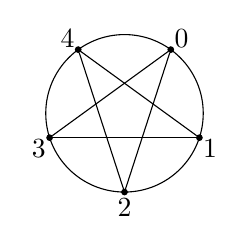
\begin{tikzpicture}[scale=1, every node/.style={draw, circle, fill=black, minimum size=2pt, inner sep=0pt}]
  \draw[black] (0,0) circle (1);

  \node (A) at (270:1) [label=below:$2$] {};
  \node (B) at (342:1) [label=below right:$1$] {};
  \node (C) at (54:1)  [label=above right:$0$] {};
  \node (D) at (126:1) [label=above left:$4$] {};
  \node (E) at (198:1) [label=below left:$3$] {};

  % ONLY diagonals (circle gives the "outer cycle" visually)
  \draw (A) -- (C);
  \draw (A) -- (D);
  \draw (B) -- (D);
  \draw (B) -- (E);
  \draw (C) -- (E);
\end{tikzpicture}
\caption{G}
\end{figure}

\begin{definition}[Graph Union]The \textit{union} of two graphs $G_{1},G_{2}$ is defined as follows.
$$G_{1}\cup G_{2}=(V(G_{1})\cup V(G_{2}),E(G_{1})\cup E(G_{2})).$$
We use $\sqcup$ to denote a union between two graphs who share no vertices (or edges).
\end{definition}
\begin{figure}[H]
    \begin{center}
        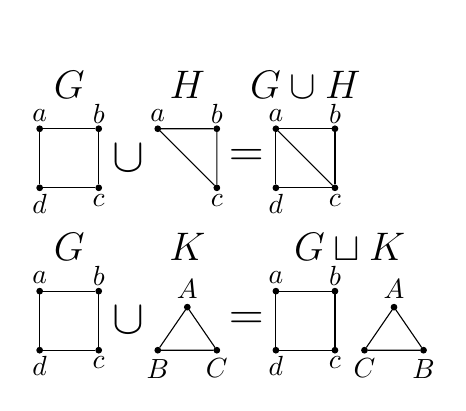
\begin{tikzpicture}[every node/.style={draw, circle, fill=black, minimum size=2pt, inner sep=0pt},scale=0.75]
            \node(G) at (0.5,0.75) [draw=none, fill=none] {\Large $G$};
            % First graph
            \node (a) at (0, 0)  [label=above:$a$]  {};
            \node (b) at (1, 0)  [label=above:$b$]  {};
            \node (c) at (1, -1) [label=below:$c$]  {};
            \node (d) at (0, -1) [label=below:$d$]  {};

            \draw (a) -- (b) -- (c) -- (d) -- (a);

            % "=" symbol
            \node[draw=none, fill=none] at (1.5, -0.5) {\LARGE $\cup$};

            % Second graph
            \begin{scope}[xshift=2cm]
                \node(H) at (0.5,0.75) [draw=none, fill=none] {\Large $H$};
                \node (a) at (0, 0)  [label=above:$a$]  {};
                \node (b) at (1, 0)  [label=above:$b$]  {};
                \node (c) at (1, -1) [label=below:$c$]  {};
    
                \draw (a) -- (b) -- (c) -- (a);
            \end{scope}

            % "\cup" symbol
            \node[draw=none, fill=none] at (3.5, -0.5) {\LARGE $=$};
            
            \begin{scope}[xshift=4cm]
                \node(GUH) at (0.5,0.75) [draw=none, fill=none] {\Large $G\cup H$};
                \node (a) at (0, 0)  [label=above:$a$]  {};
                \node (b) at (1, 0)  [label=above:$b$]  {};
                \node (c) at (1, -1) [label=below:$c$]  {};
                \node (d) at (0, -1) [label=below:$d$]  {};
    
                \draw (a) -- (b) -- (c) -- (d) -- (a);
                \draw (a) -- (c);
            \end{scope}

%second line _______________________________________________________

            \begin{scope}[shift={(0,-2.75)}]
                            % First graph
                            \node(G) at (0.5,0.75) [draw=none, fill=none] {\Large $G$};
                            \node (a) at (0, 0)  [label=above:$a$]  {};
                            \node (b) at (1, 0)  [label=above:$b$]  {};
                            \node (c) at (1, -1) [label=below:$c$]  {};
                            \node (d) at (0, -1) [label=below:$d$]  {};

                            \draw (a) -- (b) -- (c) -- (d) -- (a);

                            % "=" symbol
                            \node[draw=none, fill=none] at (1.5, -0.5) {\LARGE $\cup$};
            \end{scope}

            % Second graph
            \begin{scope}[shift={(2,-2.75)}]
                % Define coordinates so the sides are all length 2.
                \node(K) at (0.5,0.75) [draw=none, fill=none] {\Large $K$};
                \node (A) at (0.5,-0.271) [label=above:$A$]{};
                \node (B) at (0,-1) [label=below:$B$]{};
                \node (C) at (1,-1) [label=below:$C$] {};

                % Draw and label
                \draw (A) -- (B) -- (C) -- (A);
                \node[draw=none, fill=none] at (1.5, -0.5) {\LARGE $=$};
            \end{scope}

            \begin{scope}[shift={(4,-2.75)}]
                \node(GUH) at (1.25,0.75) [draw=none, fill=none] {\Large $G\sqcup K$};
                \node (a) at (0, 0)  [label=above:$a$]  {};
                \node (b) at (1, 0)  [label=above:$b$]  {};
                \node (c) at (1, -1) [label=below:$c$]  {};
                \node (d) at (0, -1) [label=below:$d$]  {};

                \node (A) at (2,-0.271) [label=above:$A$]{};
                \node (B) at (2.5,-1) [label=below:$B$]{};
                \node (C) at (1.5,-1) [label=below:$C$] {};

                \draw (a) -- (b) -- (c) -- (d) -- (a);
                \draw (A) -- (B) -- (C) -- (A);
            \end{scope}

        \end{tikzpicture}
    \end{center}
    \caption{(above)$\,G\cup H$ and (below)$\,G\sqcup K$.}
    \label{fig:unions}
\end{figure}

We say two graphs $G_{1},G_{2}$ are isomorphic if there exists a bijection $f:V(G_{1})\to V(G_{2})$ between their vertices that preserves edge structure;
$$f(a)=\alpha,\,f(b)=\beta,\text{ and }ab\in E(G_{1})\implies \alpha\beta\in E(G_{2}),\forall a,b\in V(G_{1}).$$
Graph theorists typically view all graphs in the same isomorphism class as the same graph. Another way to think of isomorphism between two graphs is through their visual representations. If you can draw one graph, and then arrange the nodes (without deleting or adding edges) so that it is identical to the visual representation of another graph, then the two are isomorphic.
\begin{figure}[H]
    \begin{center}
    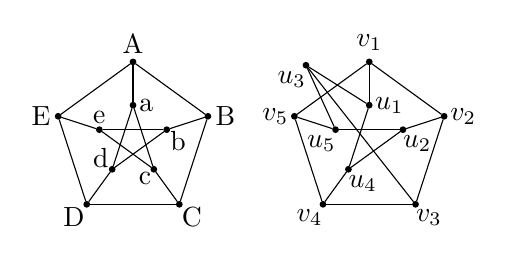
\begin{tikzpicture}[every node/.style={draw, circle, fill=black, minimum size=2pt, inner sep=0pt}]

        % Outer vertices (A,B,C,D,E)
        \node (A0) at (90:1)   [label=above:A] {};
        \node (A1) at (18:1)   [label=right:B] {};
        \node (A2) at (306:1)  [label=below right:C] {};
        \node (A3) at (234:1)  [label=below left:D] {};
        \node (A4) at (162:1)  [label=left:E] {};
    
        % Inner vertices (a,b,c,d,e)
        \node (B0) at (90:0.45)   [label=right:a] {};
        \node (B1) at (18:0.45)   [label=below right:b] {};
        \node (B2) at (306:0.45)  [label=below left:c] {};
        \node (B3) at (234:0.45)  [label=above left: d] {};
        \node (B4) at (162:0.45)  [label=above:e] {};
    
        % Outer edges
        \draw (A0) -- (A1);
        \draw (A1) -- (A2);
        \draw (A2) -- (A3);
        \draw (A3) -- (A4);
        \draw (A4) -- (A0);
    
        % Inner edges
        \draw (B0) -- (B2);
        \draw (B2) -- (B4);
        \draw (B4) -- (B1);
        \draw (B1) -- (B3);
        \draw (B3) -- (B0);
    
        % Spokes
        \draw (A0) -- (B0);
        \draw (A1) -- (B1);
        \draw (A2) -- (B2);
        \draw (A3) -- (B3);
        \draw (A4) -- (B4);

        \begin{scope}[shift={(3,0)}]
            % Outer vertices: v_1 to v_5
            \node (A0) at (90:1)   [label=above:$v_1$] {};
            \node (A1) at (18:1)   [label=right:$v_2$] {};
            \node (A2) at (306:1)  [label=below right:$v_3$] {};
            \node (A3) at (234:1)  [label=below left:$v_4$] {};
            \node (A4) at (162:1)  [label=left:$v_5$] {};

            % Inner vertices: u_1 to u_5
            \node (B0) at (90:0.45)   [label=right:$u_1$] {};
            \node (B1) at (18:0.45)   [label=below right:$u_2$] {};
            \node (B2) at (130:1.25)  [label=below left:$u_3$] {};
            \node (B3) at (234:0.45)  [label=below right:$u_4$] {};
            \node (B4) at (162:0.45)  [label=below left:$u_5$] {};

            % Outer edges (pentagon)
            \draw (A0) -- (A1);
            \draw (A1) -- (A2);
            \draw (A2) -- (A3);
            \draw (A3) -- (A4);
            \draw (A4) -- (A0);

            % Inner edges (star)
            \draw (B0) -- (B2);
            \draw (B2) -- (B4);
            \draw (B4) -- (B1);
            \draw (B1) -- (B3);
            \draw (B3) -- (B0);

            % Spokes between outer and inner
            \draw (A0) -- (B0);
            \draw (A1) -- (B1);
            \draw (A2) -- (B2);
            \draw (A3) -- (B3);
            \draw (A4) -- (B4);
        \end{scope}

    \end{tikzpicture}
\end{center}
    \caption{$\text{(left) }G\cong H \text{ (right)}$.}
    \label{fig:isomorphismexample}

\end{figure}
We wrap up the basics with some important concepts and operations needed to understand the work done in this thesis. This is an excerpt from the paper itself.
\begin{definition}[Subgraph] A subgraph $G\subseteq K$ is a graph whose vertices and edges are subsets of the vertices and edges of $K$; $G\subseteq K$ if $V(G)\subseteq V(K)$ and $E(G)\subseteq E(K)$.
\end{definition}


\begin{definition}[Vertex-induced Subgraph] A \textit{vertex-induced} subgraph $G\subseteq K$ is one whose vertices are some subset $S$ of $V(K)$ and whose edges are all edges between those vertices in $K$; $V(G)=S\subseteq V(K)$ and $E(G)=\{uv\in E(K)\mid u,v\in S\}$. If $G$ is such a subgraph we say that $G$ is induced by $S=V(G)\subseteq V(K)$.
\end{definition}
\begin{definition}[Edge-induced Subgraph] An \textit{edge-induced} subgraph $G\subseteq K$ is one whose edges are some subset of $E(K)$ and whose vertices are all those who appear as an endpoint in that subset of edges; $E(G)\subseteq E(K)$ and $V(G)=\{u\in V(K)\mid uv\in E(G)\text{ for some }v\in V(K)\}$. If $G$ is such a subgraph we say that $G$ is induced by $S=E(G)\subseteq E(K)$
\end{definition}

Here is a visual example of these types of graphs: Let $K$ be the Petersen graph from Figure 
\begin{align*}
    &\textbf{Subgraph: } \textcolor{magenta}{G} \subseteq K \text{ where }\textcolor{magenta}{V(G)} = \textcolor{magenta}{\{E, e, b\}},\; \textcolor{magenta}{E(G)} = \textcolor{magenta}{\{Ee\}}.\\
    &\textbf{Vertex-induced Subgraph: } \textcolor{blue}{H} \subseteq K \text{ is induced by } \textcolor{blue}{\{a, A, B\}}\subseteq V(K)\\
    &\textbf{Edge-induced Subgraph: } \textcolor{red}{M} \subseteq K 
    \text{ is induced by }\textcolor{red}{\{Dd, DC, Cc\}}\subseteq E(K)
\end{align*}
The figure below shows $K$ and it's color-coded subgraphs.

\begin{figure}[H]
    \begin{center}
    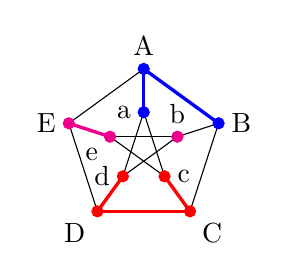
\begin{tikzpicture}[scale=1]
    
        %--- Base style for all nodes:
        \tikzstyle{base node}=[draw, circle, fill=black, minimum size=2pt, inner sep=0pt]
    
        %--- Outer vertices (A,B,C,D,E)
        \node[base node, label=above:A]         (A0) at (90:1)   {};
        \node[base node, label=right:B]         (A1) at (18:1)   {};
        \node[base node, label=below right:C]   (A2) at (306:1)  {};
        \node[base node, label=below left:D]    (A3) at (234:1)  {};
        \node[base node, label=left:E]          (A4) at (162:1)  {};
    
        %--- Inner vertices (a,b,c,d,e)
        \node[base node, label=left:a]         (B0) at (90:0.45)   {};
        \node[base node, label=above:b]   (B1) at (18:0.45)   {};
        \node[base node, label=right:c]    (B2) at (306:0.45)  {};
        \node[base node, label=left:d]    (B3) at (234:0.45)  {};
        \node[base node, label=below left:e]         (B4) at (162:0.45)  {};
    
        %--- Edges of K (in black)
        % Outer ring
        \draw (A0) -- (A1);
        \draw (A1) -- (A2);
        \draw (A2) -- (A3);
        \draw (A3) -- (A4);
        \draw (A4) -- (A0);
    
        % Inner pentagon
        \draw (B0) -- (B2);
        \draw (B2) -- (B4);
        \draw (B4) -- (B1);
        \draw (B1) -- (B3);
        \draw (B3) -- (B0);
    
        % Spokes
        \draw (A0) -- (B0);
        \draw (A1) -- (B1);
        \draw (A2) -- (B2);
        \draw (A3) -- (B3);
        \draw (A4) -- (B4);
    
        %=== Subgraph G in magenta: V(G)={E, e, b}, E(G)={Ee, eb}
        \draw[magenta, very thick] (A4) -- (B4);  % E--e
        %\draw[magenta, very thick] (B4) -- (B1);  % e--b
        \node[draw=magenta, fill=magenta, circle, minimum size=4pt, inner sep=0pt] at (A4) {};
        \node[draw=magenta, fill=magenta, circle, minimum size=4pt, inner sep=0pt] at (B4) {};
        \node[draw=magenta, fill=magenta, circle, minimum size=4pt, inner sep=0pt] at (B1) {};
    
        %=== Vertex-induced subgraph H in blue: induced by {a, A, B}
        % Edges among {a,A,B} in K are A--B and A--a
        \draw[blue, very thick] (A0) -- (A1);   % A--B
        \draw[blue, very thick] (A0) -- (B0);   % A--a
        \node[draw=blue, fill=blue, circle, minimum size=4pt, inner sep=0pt] at (A0) {};
        \node[draw=blue, fill=blue, circle, minimum size=4pt, inner sep=0pt] at (A1) {};
        \node[draw=blue, fill=blue, circle, minimum size=4pt, inner sep=0pt] at (B0) {};
    
        %=== Edge-induced subgraph M in red: induced by {Dd, DC, Cc}
        % These edges correspond to D--d, D--C, C--c in K
        \draw[red, very thick] (A3) -- (B3);    % D--d
        \draw[red, very thick] (A3) -- (A2);    % D--C
        \draw[red, very thick] (A2) -- (B2);    % C--c
        \node[draw=red, fill=red, circle, minimum size=4pt, inner sep=0pt] at (A3) {};
        \node[draw=red, fill=red, circle, minimum size=4pt, inner sep=0pt] at (B3) {};
        \node[draw=red, fill=red, circle, minimum size=4pt, inner sep=0pt] at (A2) {};
        \node[draw=red, fill=red, circle, minimum size=4pt, inner sep=0pt] at (B2) {};
    
    \end{tikzpicture}
    \end{center}
    \caption{$K$ and subgraphs $\textcolor{magenta}{G}, \textcolor{blue}{H}, \textcolor{red}{M} \subseteq K$.}
    \label{fig:subgraphs}
    \end{figure}

\begin{definition}[Graph Complement]
The complement of a graph $G$ denoted $\overline{G}$ is the graph obtained by removing all edges of $G$ and then adding in all edges not originally present in $G$. Formally, 
$$\overline{G}=(V(G), \{uv\mid u,v\in V(G) \text{ and } uv\not\in G\})$$
\end{definition}
Here is an example of a graph complement. Let $G=(\{a,b,c,d\},\{ab,bc,cd,da\})$. Then $\overline{G}=(\{a,b,c,d\},\{ac,bd\})$. These graphs are depicted in the figure below.

\begin{figure}[h]
    \begin{center}
    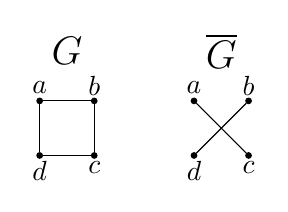
\begin{tikzpicture}[every node/.style={draw, circle, fill=black, minimum size=2pt, inner sep=0pt}, scale=0.49]
        % Place vertices to form an upward-facing pentagon
        \node(G) at (90:2) [draw=none, fill=none] {\Large $G$};
        \node (a) at (135:1) [label=above:$a$]   {};   % Top vertex
        \node (b) at (45:1) [label=above:$b$]   {};
        \node (c) at (-45:1) [label=below:$c$]  {};
        \node (d) at (-135:1) [label=below:$d$] {};
 
        % Connect vertices in cyclic order to form the pentagon (cycle graph C_5)
        \draw (a) -- (b) -- (c) -- (d) -- (a);

        \begin{scope}[xshift=4cm]
            \node(G) at (90:2) [draw=none, fill=none] {\Large $\overline{G}$};
            \node (a) at (135:1)[label=above:$a$]   {};   % Top vertex
            \node (b) at (45:1) [label=above:$b$]  {};
            \node (c) at (-45:1) [label=below:$c$] {};
            \node (d) at (-135:1) [label=below:$d$] {};

            \draw (a) -- (c);
            \draw (b) -- (d);
        \end{scope}
    \end{tikzpicture}
    \end{center}
    \caption{(left) $G$ and $\overline{G}$ (right).}
    \label{fig:complement}
    \end{figure}

\begin{definition}[Join]
    Let $G$ and $H$ be vertex disjoint graphs. Their
    \textit{join}, denoted $G \vee H$, is the graph obtained by
    taking the disjoint union of $G$ and $H$ and adding all
    possible edges between every vertex in $G$ and every vertex
    in $H$. Formally:
    $$
      G \vee H
      \;=\;
      \bigl(
        V(G)\cup V(H),
        E(G)\;\cup\;E(H)\;\cup\;\{\,xy \mid x\in V(G),\, y\in V(H)\}
      \bigr).
    $$
  \end{definition}

\begin{figure}[h]
    \begin{center}
        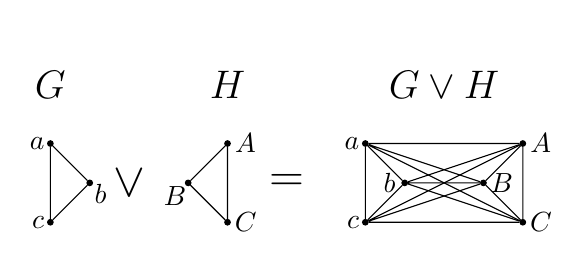
\begin{tikzpicture}[every node/.style={draw, circle, fill=black, minimum size=2pt, inner sep=0pt},scale=1]
            \node (G) at (0,0.75) [draw=none, fill=none] {\Large $G$};
            \node (a) at (0,0) [label=left:$a$]{};
            \node (b) at (0.5,-0.5) [label=below right:$b$]{};
            \node (c) at (0,-1) [label=left:$c$]{};

            \draw (a) -- (b) -- (c) -- (a) {};

            \node[draw=none, fill=none] at (1, -0.5) {\LARGE $\lor$};

            \node (H) at (2.25,0.75) [draw=none, fill=none] {\Large $H$};
            \node (A) at (2.25,0) [label = right:$A$]{};
            \node (B) at (2.25,-1)[label = right:$C$]{};
            \node (C) at (1.75,-0.5) [label = below left:$B$]{};

            \draw(A) -- (B) -- (C) -- (A){};

            \node[draw=none, fill=none] at (3, -0.5) {\LARGE $=$};

            \begin{scope}[shift={(4,0)}]
                \node (GVH) at (1,0.75) [draw=none, fill=none] {\Large $G\lor H$};
                \node (a) at (0,0) [label=left:$a$]{};
                \node (b) at (0.5,-0.5) [label=left:$b$]{};
                \node (c) at (0,-1) [label=left:$c$]{};

                \draw (a) -- (b) -- (c) -- (a) {};

                \node (A) at (2,0) [label = right:$A$]{};
                \node (B) at (2,-1)[label = right:$C$]{};
                \node (C) at (1.5,-0.5) [label = right:$B$]{};

                \draw(A) -- (B) -- (C) -- (A){};

                \draw (a) -- (A) -- (a) -- (B) -- (a) -- (C);
                \draw (b) -- (A) -- (b) -- (B) -- (b) -- (C);
                \draw (c) -- (A) -- (c) -- (B) -- (c) -- (C);
            \end{scope}
        \end{tikzpicture}
    \end{center}
    \caption{(left) $G$, $H$ (middle), and $\,G\vee H$ (right).}
    \label{fig:join}
\end{figure}

\subsection{Algebra}
Some basic algebraic machinery can simplify many of the constructions in this thesis. This area of research lies in an intersection of Graph Theory, Combinatorics, and Design Theory. Depending on the context it can be helpful to think of the objects studied in this work from many different perspectives offered by these disciplines, but the thread connecting them all, constructively anyways, is Group Actions.$\newline$

It is assumed that the reader understands knows what a group is. The only thing to cover on that front is that the group $\ZZ_{n}$ is presented as $\ZZ_{n}=\{0,1,\hdots, n-1\}$ rather than $\{[0],[1],\hdots, [n-1]\}$. This is done for the sake of hygeine.$\newline$

\noindent We now briefly define Group Actions and Orbits.
\begin{definition}[Group Action]
We say a Group $G$ acts on a set $X$, and denote that statement $G\curvearrowright S$ if there exists a mapping
$\varphi: G\times X\to X$ such that
\begin{align*}
&\textbf{[Identity]: } \varphi(e,x)=x,\,\forall x\in X\\
&\textbf{[Compatibility]: }\varphi(gh,x)=\varphi(g,(\varphi(h,x)))
\end{align*}
Notations for the actual mappings themselves can vary depending on the context. Often we use $\varphi_{g}(x)$ or $g(x)$ to denote $\varphi(g,x)$. Sometimes, we may even just denote an action using a binary operation such as $\cdot$, for example when a group is acting on one of it's subgroups.
\end{definition}
Really, all that is necessary to take away from this is that a group action permutes the elements of $X$ such that composition preserves multiplication between group elements. This allows us to essentially do some algebra with elements of sets. We only need one other concept for this research.
\begin{definition}[Orbit]
If a group $G$ acts on a set $X$, we call the set of all elements that $x$ is permuted to via $G$, the orbit of $x$:
$$\mathrm{Orb}_{G}(x)=\{g(x)\mid g\in G\}$$
\end{definition}
The next section will describe certain mappings called \textit{labelings} which prove the existence of certain types of \textit{graph decompositions}. The way they prove existence is constructively, through group actions. We could just define these labelings and call it a day since theorems say they prove existence (as many do), but that would be lame. That is like ordering a tasty intricate burger or sandwich and then asking the server to just throw it in your mouth and hammer it down your throat with a rubber mallet. We want to appreciate the sandwich, not just consume it for nutritional value.
\section{Decompositions}
Think back to our sandwich analogy in the previous section.

\end{document}
